\documentclass[10pt,twoside,a4paper]{report}
\usepackage{amsmath}
\usepackage{amsfonts}
\usepackage{amssymb}
\usepackage{csquotes}
\usepackage{caption}
\usepackage{subcaption}
\usepackage[hidelinks]{hyperref}
\usepackage[]{algorithm2e}
\usepackage{fontspec}
% ETHASL package
% TODO Choose options according to your project
% som/bt/st/mt: Studies on Mechatronics, Bachelor Thesis, Semester Thesis, Master Thesis
% fs/hs: Spring term, Autumn term
% german/english: German/English
\usepackage[bt,fs,english]{packages/ethasl}

% Activate for german language
%\usepackage{german}
%\usepackage{ae}

%%%%%%%%%%%%%%%%%%%%%%%%%%%%%%%%%%%%%%%%%%%%%%%%%%%%%%%%%%%%%%%%%%%%%%%%%%%%%%%
% LaTeX preamble
%%%%%%%%%%%%%%%%%%%%%%%%%%%%%%%%%%%%%%%%%%%%%%%%%%%%%%%%%%%%%%%%%%%%%%%%%%%%%%%
\input{preambles/asl_preamble}


\title{Path Generation for a Mobile Drawing Robot}
%\subtitle{bla bla bla}

% TODO Add name of the authors
\studentA{Wolf Vollprecht}
% \studentC{Student 3}

% TODO Add name of the supervisors
\supervisionA{Nikolay Kobyshev}
\supervisionB{Philipp Krüsi}
%\supervisionC{Supervisor C}

% TODO Change if necessary
\projectYear{\the\year}
\begin{document}

%\maketitle
\pagestyle{plain}
\pagenumbering{roman}

\author{Wolf Vollprecht}
\title{Path Generation for a Mobile Drawing Robot}

%\input{chapters/preface}
%\cleardoublepage
%\chapter*{Abstract}
\addcontentsline{toc}{chapter}{Abstract}
%\chapter*{Zusammenfassung}
%\addcontentsline{toc}{chapter}{Zusammenfassung}

The BeachBot is a mobile, autonomous drawing robot for large scale sand art. Its primary purpose is the entertainment of beachgoers. The goal of this thesis was to develop and evaluate algorithms to automatically generate suitable trajectories to draw arbitrary images on the canvas. Main challenges have been to find a trajectory that reduces the drawing time and to make watching the drawing process appealing.

%\cleardoublepage
%\input{chapters/symbols}
%\cleardoublepage

%\tableofcontents

\pagestyle{fancy}
\pagenumbering{arabic}
\chapter{Introduction}
\section{The BeachBot Project}


\section{Requirements and Inspiration}

The BeachBot project itself was inspired by the images of sand artists like Peter Donnelly and Andres Amador, who manually create large scale sand art at beaches using a rake. Some of the imagery that was found online can be seen in \autoref{fig:sandart_inspiration}.

\begin{figure}
\centering
\begin{subfigure}[c]{1\textwidth}
\includegraphics[width=\textwidth]{images/requirements_inspiration/donnelly_1.jpg} 
\caption{Sand drawing by Peter Donnelly. Source: \url{http://becky-garrett.blogspot.ch/2009/03/sand-dancer-peter-donnelly.html}}
\end{subfigure}
\\
\begin{subfigure}[b]{0.46\textwidth}
\includegraphics[width=\textwidth]{images/requirements_inspiration/andres_armador_1.jpg} 
\caption{Sand drawing by Andres Amador. Source: \url{http://sftimes.co/?id=25}}
\end{subfigure}
~
\begin{subfigure}[b]{0.46\textwidth}
\includegraphics[width=\textwidth]{images/requirements_inspiration/andres_armador_2.jpg} 
\caption{Sand drawing by Andres Amador. Source: \url{http://sftimes.co/?id=25}}
\end{subfigure}
\caption{Various beach drawings by artists}
\label{fig:sandart_inspiration}
\end{figure}

Since the goal of the project is to create drawings similar to those of the artists, the requirements were derived from these sample images.

First of all, the BeachBot should be able to draw lines. But more important is the support of filled areas. While it is relatively straightforward how to drive over lines or curves to draw them, there is no easy solution to derive the path for the filled areas. Not only should the area be covered to the highest extent, but the drawing process should also look interesting and artistic to spectators as well.

Derived from \autoref{fig:sandart_inspiration} is also the requirement that the BeachBot only needs to be able to draw in two colors. Gradients or differently colored areas are unnecessary.

Crossing lines or filled areas should be avoided as good as possible since the balloon wheels and the front wheel leave visible marks on the raked sand (a humanoid has a huge advantage here, since it can jump over the drawn areas). The effect of driving over the drawing depends on the scale. If the drawing is very big, it does not matter much if part of the image is crossed out. 

The input of the path generator should not only be computer readable, but also human editable. Typing in endless lists of coordinates would be tedious in the long run, and having a difficult format to work with would make it hard to collaborate with artists, for example. 
%Therefore the requirement to be able to use a modern graphics editor tool to work with was set. To conform to this requirement we soon decided to use \textit{Inkscape}\footnote{\url{http://inkscape.org}}, a popular open source vector graphics editor, as our input creation tool of choice. Further discussion about vector graphics as input and the steps to integrate a standardized vector graphics format into the path generator are explained in \autoref{sec:why_vector} and \autoref{sec:implementation_svg} respectively.

During the testing phase it was found out, that some of the generated paths needed some manual adjusting. To be able to easily edit the output of the generator program a graphical user interface should be created to work with the output of the generator program. 

In the following sections it will be shown how these requirements were fulfilled and to which extent.

\subsection{The Path Converter}\label{sec:pathconv}

Another bachelor thesis that was written as part of the BeachBot project deals with the rake offset of the robot. The rake is not at the same spot as the turning point of the robot, which leads to errors when the image is drawn in the sand. Therefore, the path converter uses an optimization technique to adjust the path generated by this bachelor thesis in a way that the rake closely follows the generated path by offsetting the robot trajectory. The Path Converter is introduced here because, as will later be discussed, leads to certain limitations that had to be regarded for the design of the path generation algorithms. As a matter of fact, the path that is generated in this thesis is the rake path and not the robot path.


% here you say that the project consists of a GUI and an algorithm.

\chapter{Path Planning Algorithms}
\section{Algorithm Overview}

The output of the path generator should be a single trajectory that completely connects and covers all elements of the drawing.

This happens in three steps: First, the polygons that have to be filled are selected and the fill algorithm is seperately executed for each of the polygons with polygon specific settings. In a second step all of the drawing elements are connected by an open tour and tries to minimize the traveled distance by applying a traveling salesman heuristic. As last step, connections with limited curvature are generated to complete the trajectory.

Each of those steps will be discussed in detail in this section.
% here you set the main requirements connected, as short as possible, no sharp angles etc)
\section{Image Structure}

Derived from the requirements, three different elements were identified as part of drawing (also shown in \autoref{fig:elements_def}:

\begin{description}
\item[Polyline] A line consisting of $2$ to $n$ vertices
\item[Polygon] A closed line, consisting of $2$ to $n$ vertices, where the last segment is a closing one. So that vertex $v_{n+1}$ equals $v_0$.
\item[Filled Polygon] Defined in the same way as the polygon, except that the inner space should be filled by the generated trajectory. Another difference is that the filled polygon can also contain holes, which should not be covered and be excluded from the fill trajectory.
\end{description}

\begin{figure}
\centering
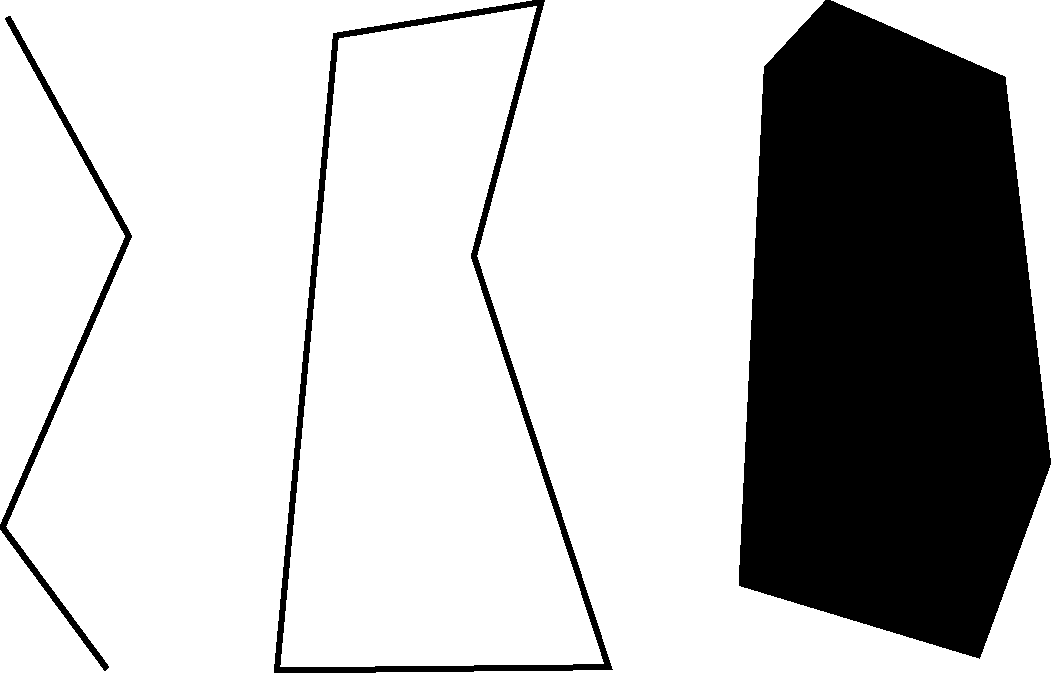
\includegraphics[width=0.6\textwidth]{images/path_planning/line_polygon_definition.pdf}
\caption{Polyline, polygon and filled polygon}
\label{fig:elements_def}
\end{figure}

% you discuss the lines, closed lines, filled polygons
% then you explain the structure that you work on elements separately and the connect them with TSP.
\section{Polygon Filling}

\subsection{Related Work}

Over time several surface coverage algorithms have been developed, and some distinctions can be made. 

Coverage algorithms exist for applications like autonomous vaccuum cleaners or autonomous lawn mowers, but also search and rescue robotic applications usually and they usually do not care if they visit the same spot twice. The target for those algorithms is rather to achieve complete coverage of an previously unknown terrain in sensible time. Usually, the complete surface coverage algorithms in are also connected with online map generation techniques \textit{SLAM}, whereas the path generation for the BeachBot should happen offline.

However, in agricultural applications some interesting algorithms have been found, which served as inspiration for the explorations presented in this thesis. Especially \citep{ROB:ROB20300}, who hinted at exploiting the straight skeleton algorithm to generate the inset polygons. An optimization strategy is employed to find the shortest trajectory through the field by repeatedly offsetting the remainding shape and traversing all possible ways off filling the shape. The algorithm is relatively computing intensive, what might be justified when using huge agricultural machines but what was not necessary for the goals of this thesis as the benefit of this optimization would be relatively small.

Another field where trajectories have to be generated is in \textit{Computer Aided Machining}. The process of removing layers of material from a block of metal is quite similar (though inverse, usually) to what is achieved in this thesis. Many publications deal with the problem of multi-axis milling machines which are far more complex and are also able to go over the machined surface without problem because they can lift the machnining head -- something that is not possible with the autonomous ground robot. 

One interesting publication in the CAM field is \cite{kao1998optimal} that presents a method to reduce gaps that are present when simply offsetting a polygon with spirals. The presented method could be a possible future improvement to the spiral fill algorithm of \autoref{sec:spiral_fill}.

The OpenCAM library has also been inspected...

	% all the algorithms go here
\subsection{Spiral Filling}

\subsubsection{Straight Skeleton}

To generate a spiral fill for the trajectory, we use the properties of the so called straight skeleton. The straight skeleton is defined as the topolgical skeleton of a polygon that is created by moving the edges inwards at a constant speed and observing the intersections of the vertices. It was first described by \citep{Aichholzer:jucs_1_12:a_novel_type_of}. 

During the creation of the straight skeleton, two events can happen: 

\begin{itemize}
\item Edge event: An edge shrinks to zero, making its neighboring edges adjacent now.
\item Split event: An edge is split, i.e., a reflex vertex runs into this edge, thus splitting the whole polygon. New adjacencies occur between the split edge and each of the two edges incident to the reflex vertex.
\end{itemize}
(cited from \citep{Aichholzer:jucs_1_12:a_novel_type_of}).

The straight skeleton is similar to the median axis of a polygon, but unlike the median axis it is not defined to have a constant distance to the polygon edges.

For the case of this thesis, the most interesting property of the straight skeleton is the ability to easily obtain inset polygons. The inset polygons are used to create a spiral fill for the polygons. The procedure is as follows:

\begin{itemize}
\item[(0)] The straight skeleton is generated
\item[(1)] The inset polygon is created
\item[(2)] If a split event has happened, then it is decided which polygon should be used to extend the current spiral (that is the one with the closer point to our current position). All the others are recursively filled in the same way. Additionally, a starting point to the spiral is passed, so that the beginning of the next spiral will be close to the current one. (The procedure restarts with the split polygon as input at (0)).
\item[(3)] The $n+1$ vertex of the inset polygon is appended to the current spiral
\item[(4)] An inset polygon is generated with inset length divided by number of vertices. Through dividing the inset length (which is predefined, usually as one rake width) by the number of vertices in the polygon, we make sure that one revolution of the spiral will travel only one rake distance.

\end{itemize}

%\begin{algorithm}[H]
%\SetKwFunction{FRecurs}{FillPolygon}
%\Fn(){\FRecurs{some args}}{
% \KwData{Polygon P, Startpoint SP, RakeWidth}
% \KwResult{Single trajectory}
% CurrPoint = findNearestPoint(SP, P)\;
% CurrOffset = RakeWidth / P.numberVertices\;
% S = generateStraightSkeleton(P)\;
% O = generateOffsetPolygons(CurrOffset, S)\;
% \While{$O.numberOfPolygons > 0$}{
%  \If{$O.numberOfPolygons > 1$} {
%	P = findCloserPolygon(O, CurrPoint)\;
%  }
% }
% \caption{How to write algorithms}
%\end{algorithm}

The algorithm is both displayed in pseudo code and graphically. 

\begin{figure}[htbp]
	\centering
    \begin{subfigure}[b]{0.45\textwidth}
    		\includegraphics[width=\textwidth]{images/algorithms/spiral_fill/2.pdf}
		\caption{The first inset polygon and the first part of the spiral line}
    \end{subfigure}
    ~
    \begin{subfigure}[b]{0.45\textwidth}
    		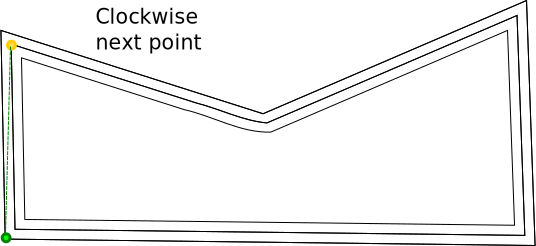
\includegraphics[width=\textwidth]{images/algorithms/spiral_fill/3.pdf}
    		\caption{Next inset polygon generated}
    \end{subfigure}\\
    \begin{subfigure}[b]{0.45\textwidth}
    		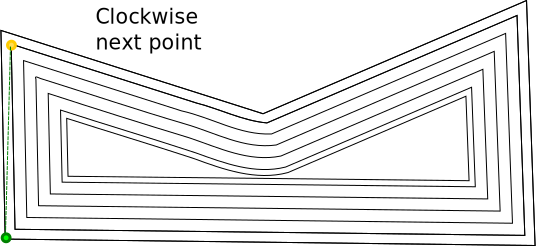
\includegraphics[width=\textwidth]{images/algorithms/spiral_fill/4.pdf}
    		\caption{The polygon right before the \textit{split} happens}
    \end{subfigure}~
    \begin{subfigure}[b]{0.45\textwidth}
    		\includegraphics[width=\textwidth]{images/algorithms/spiral_fill/done.pdf}
    		\caption{After split, next polygon was found for continuing the current spiral}

    \end{subfigure}
        \begin{subfigure}[b]{0.45\textwidth}
    		\includegraphics[width=\textwidth]{images/algorithms/spiral_fill/after_done_2.pdf}
    		\caption{Continuing spiral 1 and starting the second spiral. Note how the start point of the second spiral is the closest point to the endpoint of the first.} \label{splitevent}
    \end{subfigure}
\\
        \begin{subfigure}[b]{0.45\textwidth}
    		\includegraphics[width=\textwidth]{images/algorithms/spiral_fill/complete_done.pdf}
    		\caption{The completed spiral with all inset polygons removed.}
    \end{subfigure}
	\caption{Generating the fill spiral. Note that this is only an example for illustration purposes. Of course, the density of inset polygons for a real application is much higher.} \label{fig:insetting}
\end{figure}

\begin{figure}
\centering
\includegraphics[width=0.6\textwidth]{images/algorithms/spiral_fill/spiral_real.pdf}
\caption{Generated spiral} \label{fig:gen_spiral}
\end{figure}

\subsection{Back and Forth Filling}

This fill method is quite straight forward: The polygon is filled by a number of lines that are parallel to each other and clipped at the polygon edges. 
	% your algorithm. \subsubsection{Optimal Convex Partitioning} goes here without a special subsection for it

\section{Path Generation}
As already mentioned, to finally create a drawing all elements have to be connected by support trajectories where the rake is lifted. The supporting paths should have two properties: The total sum of all support paths should be as small as possible and the curvature of the connections should be limited.

As previously defined, a drawing consists of the three different types: Lines, polygons and filled polygons. Lines and polygons differ in the way they can be connected, as illustrated in \autoref{fig:connect}. A line can be entered or exited on both ends and is traversed in a previously unknown direction. A polygon however can be entered at any vertex, but can only be exited at the same so that the polygon is closed. Filled polygons work the same as the regular polygon in that sense, since the spiral and the back and forth filling create a polyline that is inserted into the filled polygon.

\begin{figure}
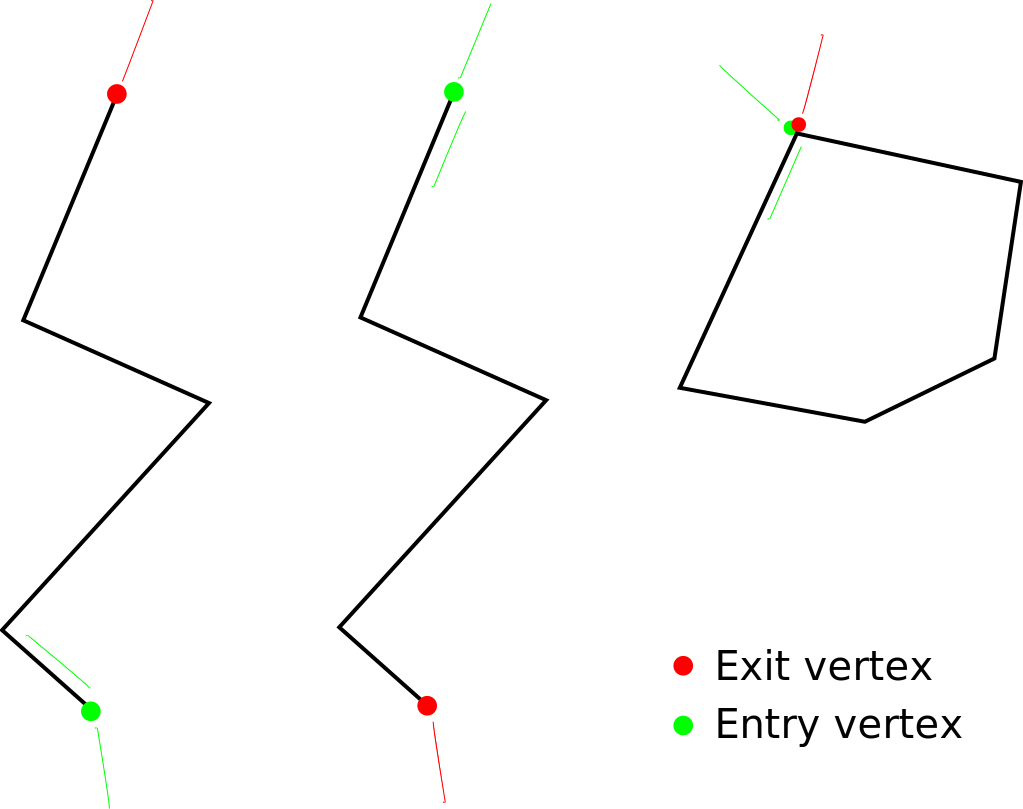
\includegraphics[width=0.8\textwidth]{images/path_planning/traversal.pdf}
\caption{Possible entry- and exit vertices and direction of traversal for polylines and polygons. Note that the polygon could also be traversed in clockwise direction.}
\end{figure}

\subsection{Traveling Salesman Problem}

The Traveling Salesman Problem (TSP) is the problem of finding the minimum-weight Hamiltonian Circuit in a weighted graph. A weighted graph is a graph where every edge between two vertices has a certain weight. The Hamiltonian Circuit is defined as a tour through the graph, that travels to every vertex exactly once. It is called salesman problem because in the historical context the vertices were cities and the salesman, seeking to minimize the distance traveled to visit all the cities in a given tour, would have liked to get a solution for this problem. However, one of the properties that make this problem hard is that it is NP-hard. If no heuristic is used, the amount of solutions that have to be searched in order to test all available possibilities is $n!$.

The TSP can be subcategorized in three categories: 

\begin{description}
\item[Symmetric] A TSP is symmetric if all distances between every node pair are symmetric (equal) in both directions from $A \leftrightarrows B$.
\item[Metric] In a metric traveling salesman problem, all distances conform to the triangle inequality $c \leq a + b$ which is, for example, true if all distances are calculated using the euclidean distance formula between two points: $\overline{AB} = \sqrt{(x_1 -x_2)^2 + (y_1 - y_2)^2}$ but also for the so called Manhattan distance which is defined as $\overline{AB_M} = |x_1-x_2| + |y_1 - y_2|$.
\item[Asymmetric] If the weights are different from $A \rightarrow B$ than from $B \rightarrow A$ then the TSP is assymetric. Of course, the triangle inequality cannot be fulfilled anymore.
\end{description}

The simplest heuristic to the TSP is the nearest neighbour search. From a given startpoint the nearest, unvisited vertex is searched and connected. This is done until no more unvisited elements exist. Positive about the nearest neighbour approach is that the complexity is only growing linear to the search size. However, the obtained solutions are often of unsatisfying quality.

Another popular heuristic is the branch and bound method. It works by splitting the set of possible solution into two halves and calculating a upper and lower bound for both. If the upper bound of the first is lower than the lower bound of the second, the second is discarded. During the course of this thesis a variant of the depth-first branch and bound search was implemented. First, the graph was traversed until a tour was completed. Afterwards, another tour (in order) was recursively started. As soon as the traveled distance of the entire tour in that branch got higher than the current minimum tour, the branch is discared. While this already reduces the search space, the effect becomes relatively small on larger problems (e.g. the first 6 out of 15 nodes might only seldomly span a tour which distance is higher than the current minimum, and it gets only worse).  It must be said, that the implementation was not very mature, and it actually produces an optimal tour in the current implementation, which is not desired in a heuristic. With more level-wise bounds it could have been a lot more efficient. 

The final solution to the minimum connection problem was to use a state of the art TSP solver\cite{helsgaun2000effective}, which employs the Lin-Kernhighan-Heuristic\cite{kernighan1970efficient} (LKH) to approximately solve the Traveling Salesman Problem. It is, unlike many other TSP solver implementations that require the triangle inequality to hold, also well suited to solve assymetric problems.
% general definition
% all three methods we tried, including LKH
\subsection{Adaptation of Traveling Salesman Problem for the Algorithm}

To find a suited tour with the generic LKH solver, the correct weights for the graph have to be specified. This happens in logical steps:

\begin{itemize}
\item On polylines, all vertices that are not the first or last node are removed, since they can never be accessed without entering at either the first or last node 
\item Polygons can be entered at any node. However, once entered, the polygon cannot be exited at any location but most be traversed completely. To enforce this, the weights on the polygon edges are set to be zero for the next vertex in clockwise direction and infinity in for all other nodes of the polygon.
\item Every node is only visited once. This leads to problems in polygons, where the tour should be closed. There are two possible solutions: Double cities or weight shifting. Since the double cities approach is doubling the number of cities it is clearly the less optimal approach. Because it is known that entering at node $n$ will result in the visitor ending up at node $n-1$ (all edges are zero), using the weight shifting method, the outgoing weights of the polygon at node $n$ are shifted to node $n-1$. Thereby, the elementwise symmetry is restored and a optimal solution can be found with a generic TSP solver. In a post processing step, the polygon is closed again.
\item All other edge weights are the euclidean distances between the vertex pair
\end{itemize}

A regular TSP tour is closed. This implies that a regular tour has a tendency to go back to the starting point after diverging into another direction at the beginning. The solution that was found is to enforce a defined start point to be inserted. The outgoing weights of the start point are either euclidean distances or defined to be the same to every node in the graph. If they are euclidean, chances are very high that the starting line is the nearest neighbour. If the outgoing weights are all defined to be $1$ the LKH can find the best suited start point on it's own because the startpoint will not induce any preference for any of the nodes.

The ingoing weights for the startpoint are chosen to be equal for all nodes. Thus, the TSP will never optimize towards traveling back to the start point.

\section{Smooth Line Connections}

While not required by the robot kinematics of the BeachBot (which can turn on the spot), generating smooth connections is beneficial to the path converter that translates the generated rake path into a robot path that is drivable by the bot. If the curvature at a given point in the connection is too high, it is not possible for the path converter to find a converging solution which makes tedious manual work needed to adjust the curvature of the connections until the converter is able to find a solution. The rounded connections would also create a nice visual effect for spectators.

Ideally a way would have to be found that limits the curvature of the connection path.

Curvature is defined as the inverse of the radius of the circle that the tangent produces at any given point in the curve. For a two dimensional curve, the curvature $\kappa$ is defined as 
$$\kappa = \frac{|x'y''-y'x''|}{(x'^2+y'^2)^{3/2}}$$


\subsubsection{Beziér Splines}

A first approach to generate more curved connections was to use Beziér splines.
The start- and endpoint of the beziér spline is trivially found as the start- and endpoint of the connection. As first solution, we used beziér splines of 3rd order. Beziér splines of 3rd order only yield 2 control points, which can, by moving them along the desired tangent, easily be used to create a connection that is smooth in the start and endpoint. However, the curvature for the complete curve can not be set because the two control points offer to few degrees of freedom. A beziér curve of 5th degree (quintic) has enough DOF to constrain the connection in terms of curvature.

The quintic Beziér curve consists of 6 control points $P_0 ... P_5$ that define the shape of the curve. $P_0$ and $P_5$ are trivially chosen because they coincide with the start- respectively the endpoint of the curves that should be connected. $P_1$ and $P_4$ are also easy to choose as they have to lie on the tangents of the curves that should be connected. $P_2$ and $P_3$ on the other hand are more difficult to obtain. Even after an extensive search through available literature it remained unclear if an analytical solution to this problem can be found or not, since the equation for curvature is getting quite complicated if expanded. In \cite{doi:10.1137/1.9781611971521.ch5} three approaches to generate beziér splines with monotone curvature are discussed. \cite{choi2010piecewise} uses piecewise 3rd degree bezier curves to create a curvature and corridor constrained trajectory.  [to be expanded]

\subsubsection{Spiro Splines}

Spiro splines, introduced by \cite{levien2009spiral} are a different approach to designing fair curves, initially for the purpose of designing fonts. They have several properties which make them well-suited for the task at hand:

They offer 4 different control points to control the shape of the curve. In contrast to beziér curves, spiro spline control points are always passed by the generated curve, whereas the bezier curve only goes through the first and last control point. The 4 different control points, denoted by a single character, of spiro splines are:

\begin{itemize}
\item[\texttt{v}] Corner point
\item[\texttt{c}] A $G^2$ continous constraint. The curvature  on the left side is the same as on the right side ($\kappa_l = \kappa_r$).
\item[\texttt{o}] Similiar to \texttt{c}, a $G^4$ continous constraint. Not only $\kappa_l = \kappa_r$ is true, but also the first and second derivative of the curvature is constrained ($\kappa_l' = \kappa_r'$, $\kappa_l'' = \kappa_r''$).
\item[\texttt{[}] A straight-to-curved control point that acts like a tangent constraint in this case.
\item[\texttt{]}] A curved-to-straight control point that also acts like a tangent constraint here.
\end{itemize}

The author, Raph Levien, has licensed his implementation \footnote{libspiro: \url{http://www.levien.com/spiro/} } of spiro splines under the GPLv2, which makes it possible to be used by this thesis. The implementation is capable of being used for realtime editing. That guarantees that the curve generation would not be the bottleneck of the application in terms of time consumption. The output of the library is a set of Beziér curves which are easier to handle in regular graphics programs.



\chapter{Implementation}
\section{Input}	% svg files, why vector is better than raster
For the implementation of the presented algorithms a input format had to be specified. As already mentioned in the requirements, it was desired that the input would be easy to edit for artists. That implies that a proper editing tool should be available. To create drawings basically two types of representation are existing: Raster images and vector graphics. Raster images work on a \textit{pixel} basis. Each pixel is saved as respective color value depending on the color space (grayscale, indexed or RGB are common). Lossy compression for raster images is available. Scaling raster graphics is limited by the resolution the image was saved in.

In contrast, vector graphics have infinite resolution because they define the image in terms of mathematical functions. Vector graphics contain information about seperate elements where raster graphics do only contain color information and don't have any concept of \enquote{element}. That makes it easy to retrieve and store metadata and, for example, parse the color of a line or area.

Due to the mentioned points it was easy to decide that vector graphics will be used as input for the path generator program. Several excellent editors are existing, such as Inkscape, which was already mentioned in the beginning, or Adobe® Illustrator®, which basically is a graphics industry standard.

Since vector graphics is only the concept a file format had to be specified as well. A number of proprietary formats, like the Adobe® Illustrator® format (\texttt{.ai}) are available, but because of their proprietary nature were ruled out. The most widely supported format for vector graphics is the Scalable Vector Graphics (SVG) specification, which is an open standard format, defined by the SVG Working Group\cite{svgstandard}. Rendering SVG is supported in all major web browsers and most modern user interface toolkits such as QT or GTK+. SVG is based on the Extended Markup Language (XML), for which a number of proprietary and open source parsers are available, thus making it easy to build upon.

\section{SVG Parser}

The main part of the SVG specification that we needed to implement is the path parsing. A path, in SVG, is represented by a sequence of commands. A command is a lower- or uppercase letter followed by a list of coordinates
\footnote{\url{http://www.w3.org/TR/SVG/paths.html}}. Coordinates following uppercase letters indicate \textit{absolute} coordinates and lowercase letter are followed by \textit{relative} coordinates. It is stateful in the way that for correct parsing the previous coordinate has to be known, except for the \texttt{M} (Move To) command.

A not complete list of possible commands is listed below:

\begin{description}
\item[\texttt{[M/m] (x,y)+}] Move To command. Starts a new (sub-)path at x,y.
\item[\texttt{[L/l] (x,y)+}] Line To command. Draws a straight line from the previous coordinate to the current coordinate.
\item[\texttt{[C/c] (x1, y1, x2, y2, x3, y3)+}] Curve To command. Defines a cubic Beziér curve with 4 control points.
\item[\texttt{Z}] Closes the element.
\end{description} 

The SVG Parser is implemented in the Python programming language. After an initial attempt to use an implementation by ourselves, it reached a certain limit of complexity that was needed to deal with output produced by Inkscape, and a rewrite would have been imminent. Our implementation did not pay respect to elementwise transforms nor to inheritance of group transforms, where a parsing tree structure would be needed. Luckily, a good implementation of all necessary features for the path generation was found online, called \enquote{svg} \footnote{\url{https://github.com/cjlano/svg}}.

It was enhanced by an attribute parser and some smaller changes to the inner workings were made to produce the necessary output. The SVG parser also has functions to reduce the Beziér splines to polygon by evaluating the polynomial at certain intervals of $t$. The resulting points are not equally spaced, which is a property of Beziér curves.

A wrapper script was created that exports two functions to the main path generator and passes the parsed objects.

\section{Tree Container}
\section{Preprocessing}
\section{Implementation of the Algorithms}
\section{Postprocessing}
\section{User Interface}

\chapter{Conclusion}
\cleardoublepage

\appendix
\chapter{Appendix}
\label{sec:appendix}
\section{Installation}

The installation procedure for the installation of the path generator program under Ubuntu 14.04 is described below:

\begin{enumerate}
\item For running the application, the following dependencies have to be satisfied:
\texttt{libcgal-dev, libboost1.54.0-all-dev, python2.7, libpython2.7-dev, build-essential, libeigen-dev, libjsoncpp-dev}. If the QT frontend should be installed, \texttt{libqt4-dev} has to be available. To be able to run the python server, the \texttt{flask} python library needs to be installed.
\item Cloning the source code from \url{https://github.com/asl-beachbot/pathmaker}: \texttt{git clone https://github.com/asl-beachbot/pathmaker}.
\item Running \texttt{cmake} with configuration options: \texttt{-DNOGUI=[ON/(OFF)]}, \texttt{-D32BIT=[ON/(OFF)]}. Round brackets indicate default value.
\item If \texttt{cmake} was run successfully, \texttt{make} can produce either the python module by using the target \texttt{python/beachbot\_pathgen} or the standalone target, called \texttt{svg\_parser} by calling e.g. \texttt{make svg\_parser -j3}.
\item If python version was built, starting the python server by calling \texttt{python python/server.py}.\\
If standalone version was built, \texttt{./svg\_parser} will launch the standalone program.
\item The HTML interface is accessed by opening the file \texttt{interface/index.html} in a recent version of the \textit{Firefox} or \textit{Chromium} web browser (server has to run).
\item To change the drawing that is opened by the server, change the file \texttt{assets/fill\_test.svg}. All sample files are also located at \texttt{assets/*.svg}.
\end{enumerate}
\newpage
\paragraph{Command Line Flags}
Command line flags can either be set as flags when the program is executed or can be set in the config file (the default file is \texttt{config.cfg} and \texttt{pythoncfg.cfg} for the server).
The list of allowed options is:
\small \\
\texttt{
  -h [ --help ]                        produce help message\\
  -f [ --filename ] arg                SVG File for parsing\\
  -r [ --round\_radius ] arg            set radius for corner rounding\\
  -m [ --fill\_method ] arg             set fill method (1: wiggle or 2: spiral)\\
  -s [ --scale\_for\_disp ] arg          scale for display\\
  --angle\_step arg                     Interpolation stepsize for rounding \\
                                       (e.g. 0.2 * PI)\\
  -m [ --max\_interpol\_distance ] arg   Max distance for points \\
  -d [ --display ]                     Open up the QT Window for inspection\\
  -t [ --threshold\_round\_angle ] arg   Defines from which angle on it should be rounded (or outer rounded)\\
  -l [ --line\_distance ] arg           Line distance inside filled elements\\
  --area\_deletion\_threshold arg        Maximum area of filling elements that will get deleted \\
  -c [ --config\_file ] arg             Use a different config file\\
  --segmentation\_on arg                Turn on or off segmentation\\
  --text\_export\_filename arg          Filename for export to textfile\\
  --svg\_export\_filename arg            Filename for export to SVG File\\
  --field\_width arg                    Width of field\\
  --field\_height arg                   Height of field\\
  --field\_offset arg                   Offset (margin) of field\\
  --segment\_offset arg                 Offset of Segment (from partitioning)\\
  --no\_tree\_ordering  Disables ordering of the tree (Useful when manual image from Timo!)\\
  --number\_segments\_bezier\_connect arg Define the number of segments for bezier interpolation)\\
  --stop\_go\_outer                      Round (and outer round) outer contours
                                       or stop-turn-go cycle?\\
  --round\_connection\_threshold         Threshold for rounding connections 
                                       (otherwise just place point) [squared 
                                       length of point distance]
}
\normalsize
\cleardoublepage

\bibliographystyle{ieeetr}
\bibliography{bibliography/references}
\addcontentsline{toc}{chapter}{Bibliography}

\end{document}
